\documentclass{book}
\usepackage[nottoc,notlot,notlof]{tocbibind}
\usepackage[spanish,mexico]{babel}
\usepackage[utf8]{inputenc}
\usepackage[T1]{fontenc} 
\usepackage{graphicx}
\usepackage{amsmath}
\usepackage{ragged2e}
\usepackage{hyperref}

%\usepackage{pslatex}
%\title{\Huge Tesis}
%\author{Alonso Baruk Brambila Rojas and Aurelio Adair Fernandez Santiago}
%\date{\today}

\usepackage{etoolbox}
\makeatletter
\patchcmd{\chapter}{\if@openright\cleardoublepage\else\clearpage\fi}{\clearpage}{}{}
\makeatother

\begin{document}
%\maketitle
\frontmatter
	\begin{titlepage}
		
		\begin{center}
			\vspace*{-1in}
			\begin{figure}[htb]
				\begin{center}
					
\includegraphics[width=10cm]{logo2}
				\end{center}
			\end{figure}
			
			FACULTAD DE INGENIERÍA ELECTROMECÁNICO\\
			\vspace*{0.75in}
			\begin{huge}
				\textsc{Desarrollo de un marco metodológico para la gestión eficiente de proyectos de Ingeniería de software}\\ %Histórico
			\end{huge}
			\vspace*{0.2in}
			\begin{Large}
			    Tesis para obtener el titulo de\\
				\textbf{Ingeniero de Software} \\
			\end{Large}
			\vspace*{0.3in}
			\begin{large}
				Presenta:\\
			\end{large}
			\begin{large}
				\textbf{Alonso Baruk Brambila Rojas}\\
				\textbf{Aurelio Adair Fernandez Santiago}\\
			\end{large}
			\vspace*{0.3in}
			\begin{large}
				Asesor:\\
			\end{large}
			\begin{large}
				\textbf{David Burguete Anguiano}\\
			\end{large}
			\vspace*{0.3in}
			\begin{large}
				Coasesor:\\
			\end{large}
			\begin{large}
				\textbf{M.C. Fernando Tomas Diaz Gárcia}\\
			\end{large}
			\vspace*{0.3in}
			%\rule{80mm}{0.1mm}\\
			\vspace*{0.1in}
			\begin{large}
				Manzanillo, Colima, México, Junio 2024.
			\end{large}
		\end{center}
		
	\end{titlepage}
\pagestyle{empty}	

\section*{Agradecimientos}

\tableofcontents
\listoffigures
\listoftables
\mainmatter

\section{Introducción}
	El desarrollo de software es un proceso complejo que se debe de realizar con precisión
planificando cada paso para lograr un resultado que cumpla con las expectativas
solicitadas. A lo largo del tiempo, se han creado diversas metodologías para guiar este
proceso, cada una con sus propias ventajas y desventajas.
Las metodologías tradicionales, como el modelo en cascada o el modelo en espiral, se
caracterizan por ser rígidas y secuenciales. Estas metodologías pueden ser útiles para
proyectos bien definidos y con requisitos estables, pero no son tan flexibles para adaptarse
a cambios o nuevas necesidades.
Por otro lado, las metodologías ágiles, como Scrum o Kanban, se basan en un enfoque
incremental e iterativo. Estas metodologías son más flexibles y adaptables a cambios, pero
pueden requerir una mayor disciplina y compromiso por parte del equipo de desarrollo.
Dado todo esto, se pretende crear una nueva metodología dirigida al desarrollo de software
que ayude a los equipos de trabajo a llevar a cabo las tareas de manera eficiente, escalable
y flexible combinando las mejores prácticas de las metodologías tradicionales y ágiles.
 
\chapter{Análisis de la problematica}

\section{Planteamiento del Problema}
	Las metodologías actuales si bien, son muy buenas y han mostrado que en su gran mayoría
funcionan, siempre existen desperfectos que la hacen que no funcionen al 100\% para todas
las personas, el objetivo de esta tesis es determinar qué conjunto de herramientas y formas
de trabajar (marco metodológico) es el ideal para que pueda existir una mejor comunicación
entre los clientes, programadores y project managers, así mismo, prometiendo entregar
software de calidad, de tal forma que cada parte del proyecto se sienta realizada y
satisfecha en cada punto del ciclo de vida del software, tratando de cumplir con todas las
expectativas que tengan cada parte de los equipos que involucran un proyecto de desarrollo
de software.
	
\section{Hipótesis}
	Se pretende crear una metodología ágil en base al continuo despliegue, para así evitar
problemas de entrega del proyecto con los clientes. Se mostrarán versiones preliminares en
etapas tempranas del proyecto, creemos que este feedback continuo nos ayudará a
entender sus necesidades en cada fase del proyecto. Para conseguir esto se necesita tener
una comunicación directa entre los desarrolladores y los clientes.
Realizamos una encuesta a personas que desempeñan deberes en una empresa de
desarrollo de software, la mayoría de las respuestas vienen de los programadores de las
empresas; con esto, se puede concluir que la gran mayoría de los involucrados en esta
encuesta buscan que la metodología sea aún más específica con el objetivo de estandarizar más los procesos, también lo que se puede rescatar de esta encuesta es que la gran
mayoría de las personas utilizan Scrum en su empresa seguido de la metodología Kanban,
sin lugar a dudas Scrum es un estándar en la industria, no obstante, otra idea que se puede
recuperar de esta encuesta es que, todos los encuestados no tendrían problemas en
aprender o aplicar una nueva metodología siempre y cuando prometa tener mejores
resultados y mejore la comunicación del equipo sin importar en qué área o qué tipo de
tecnologías estén utilizando.

\section{Objetivos}
	\subsection{Objetivo general}
	\begin{itemize}
		\item Superar las expectativas que tenemos acerca de las metodologías ágiles actuales desarrollando una nueva metodología para el desarrollo de software que permita la
		entrega de productos de alta calidad.
	\end{itemize}
	
\subsection{Objetivos específicos}
	\begin{itemize}
		\item Beneficios y carencias de las actuales metodologías ágiles
		\item Desarrollar los pasos de una metodología ágil para un desarrollo de software
		\item Probar la metodología en campo, mejorar la forma de desarrollar tareas
		\item Establecimiento de etapas para el desarrollo de una metodología ágil
		\item El desarrollo del software se realizará por un equipo multidisciplinario, con roles y responsabilidades bien definidas.
	\end{itemize}
	
\section{Pregunta de investigación}
	¿Cómo se puede mejorar el proceso de desarrollo de software?
¿Qué tan dispuestas están las personas en aprender una nueva metodología?
	
\section{Justificación}
	Los motivos que nos llevan a la creación de esta nueva metodología enfocada en los
procesos de desarrollo de software se basan en los comentarios y críticas hechas por los
desarrolladores dentro de la industria del software ya que aunque aún asi que existan
metodologías en la actualidad, estas solo se utilizan parcialmente en el desarrollo de
software, además la comunicación que existe entre el “project manager” y los
desarrolladores no siempre es la mejor, lo cual genera que los tiempos de entrega se
lleguen a aplazar y que el producto entregado no sea de la mejor calidad. Con esta nueva
metodología se busca reducir estos problemas mejorando la comunicación y el despliegue
del software desarrollado.

 
	
\chapter{Fundamentación teórica}
	Antes de que existieran las metodologías ágiles, el desarrollo de software era algo totalmente empírico y artesanal, el origen de las metodologías ágiles surge gracias a una necesidad de resolver la inconformidad de los clientes y usuarios con el software comisionado, ya que sus necesidades no estaban definidas con claridad en una fase de análisis previo, por lo que terminaban entregando sistemas que no cumplían con las expectativas de los clientes.

Antes de abordar para hablar de las metodologías ágiles primero tenemos que hablar sobre
las metodologías tradicionales, las cuales consistían en 4 puntos principales: proceso lineal y secuencial cada fase debe completarse antes de pasar a la siguiente etapa, tienen fases definidas, se divide el proyecto en fases como por ejemplo, investigación, especificaciones, diseño, desarrollo y pruebas finales, requisitos estáticos, los requisitos se capturan al principio y no se esperan cambios significativos durante el proyecto, y por el último el cuarto punto: experiencia y estabilidad, funciona bien aplicar estás metodologías en proyectos predecibles o cuando se tiene mucha experiencia en el dominio, uno de los ejemplos más conocidos en las metodologías tradicionales es la metodología waterfall (cascada).

En su contraste las metodologías ágiles tienen un enfoque iterativo, las metodologías ágiles son iterativas, se trabajan en ciclos cortos (sprints), y se adapta según el progreso. Flexibilidad y adaptabilidad, se centran en la colaboración, la flexibilidad y la entrega continua. Participación activa del equipo: el equipo de desarrollo incluído el equipo de pruebas, siempre está involucrado desde la definición de requisitos hasta la entrega, y por último el cuarto punto, iteración con el cliente, permiten una interacción directa con el usuario final.

Según \cite{Maida2015}, las primeras prácticas de desarrollo no obedecían a una metodología, los llamados programadores se abocaron a desarrollar sus códigos una vez que comprenden los requerimientos de sus clientes. Los desarrolladores en software se enfocan más en programar, que en definir los requerimientos de los clientes, haciendo antes un análisis profundo de sus necesidades. “Ante esta perspectiva se vio la importancia del análisis y del diseño en el desarrollo de un sistema. Ahora se empieza a hablar de analistas programadores y analistas de sistemas.” \cite{Carballar2009}; Durante la década de los 90, se observó la aplicación de metodologías tradicionales en proyectos que requerían respuestas rápidas y tenían requisitos poco definidos. Esta práctica generó ineficiencias, ya que se prioriza el diseño detallado y la documentación extensa en lugar de la capacidad de adaptación a posibles modificaciones en las especificaciones. Como consecuencia, surgió la necesidad de adoptar un enfoque más flexible y adaptable en el desarrollo de software.

\section{Metodologías ágiles}

\subsection{Scrum}
Scrum es una metodología ágil de gestión de proyectos que se centra en la entrega iterativa e incremental de productos. Se organiza en ciclos de trabajo llamados "sprints", que generalmente tienen una duración de 2 a 4 semanas, durante los cuales se desarrolla un conjunto de funcionalidades prioritarias del producto. Scrum se basa en roles definidos, como el Scrum Master, el Product Owner y el Equipo de Desarrollo, y utiliza artefactos como la lista de productos, la lista de tareas pendientes (backlog) y las reuniones diarias de seguimiento (daily scrum) para garantizar la transparencia, la inspección y la adaptación en el proceso de desarrollo.

\subsection{Kanban}
	Kanban es una metodología visual de gestión de proyectos que se basa en el uso de tableros visuales para representar el flujo de trabajo. Se utilizan tarjetas para representar las tareas o elementos de trabajo, que se mueven a través de diferentes columnas en el tablero según su estado. Kanban se centra en optimizar el flujo de trabajo, limitar el trabajo en progreso y mejorar continuamente el proceso de desarrollo. No tiene roles predefinidos ni ciclos de tiempo fijos, lo que lo hace altamente adaptable a diferentes contextos y tipos de proyectos.

\subsection{Extreme Programming (XP)}
	Extreme Programming (XP) es una metodología ágil de desarrollo de software que se centra en prácticas de ingeniería de software para mejorar la calidad del código y la productividad del equipo. Se basa en valores como la comunicación, la simplicidad, la retroalimentación y el coraje. XP utiliza prácticas como la programación en parejas, las pruebas automatizadas, la integración continua y la programación orientada a pruebas (TDD) para garantizar la entrega de software de alta calidad de manera rápida y sostenible.

\subsection{Lean Software Development}
	Lean Software Development es una metodología que se inspira en los principios del Lean Manufacturing para eliminar el desperdicio, optimizar el flujo de trabajo y maximizar el valor entregado al cliente. Se centra en la entrega continua de productos de alta calidad, la eliminación de procesos que no agregan valor y la mejora continua del proceso de desarrollo. Lean Software Development se basa en siete principios fundamentales, incluida la maximización del trabajo no realizado, la entrega rápida, la construcción de integridad y la optimización del todo.

\subsection{Dynamic Systems Development Method (DSDM)}
	Dynamic Systems Development Method (DSDM) es una metodología ágil de desarrollo de
	sistemas que se centra en la entrega rápida y flexible de productos que satisfagan las necesidades del negocio. Se basa en principios como el compromiso empresarial, la entrega incremental, la colaboración y la comunicación continua. DSDM utiliza una serie de fases y roles definidos, como el patrocinador del proyecto, el equipo de desarrollo y el facilitador del proceso, para garantizar la entrega exitosa de proyectos dentro del tiempo y el presupuesto acordados.

\subsection{Crystal}
	Crystal es una familia de metodologías ágiles que se adaptan a diferentes contextos y
	tamaños de proyectos. Se centra en valores como la comunicación, la simplicidad, la
	retroalimentación y la mejora continua. Crystal utiliza diferentes prácticas y procesos según el tamaño y la criticidad del proyecto, con el objetivo de maximizar la productividad y la calidad del equipo.

\subsection{Feature Driven Development (FDD)}
	Feature Driven Development (FDD) es una metodología ágil de desarrollo de software que se centra en la entrega de funcionalidades específicas y concretas en lugar de en ciclos de tiempo predefinidos. Se basa en la identificación de características clave del producto y en la división del desarrollo en fases que se centran en la entrega de estas características. FDD utiliza roles definidos, como el gerente de proyecto, el diseñador jefe y el programador de funciones, y técnicas como la inspección de modelos y la construcción por pasos para garantizar la calidad y la eficiencia en el desarrollo.

\subsection{Agile Unified Process (AUP)}
	Agile Unified Process (AUP) es una metodología ágil que combina los principios de la agilidad con las mejores prácticas de ingeniería de software. Se basa en una serie de fases iterativas y evolutivas, que incluyen la concepción, la elaboración, la construcción y la transición. AUP utiliza artefactos como modelos arquitectónicos, casos de uso y listas de tareas pendientes para guiar el desarrollo del proyecto y asegurar la calidad del producto final.

\subsection{Adaptive Software Development (ASD)}
	Adaptive Software Development (ASD) es una metodología ágil que se centra en la
	adaptabilidad y la flexibilidad para responder a los cambios en los requisitos del proyecto. Se basa en la colaboración entre el equipo de desarrollo y los stakeholders para identificar y priorizar las características clave del producto. ASD utiliza técnicas como el desarrollo evolutivo, la planificación adaptativa y la entrega incremental para garantizar la entrega oportuna y efectiva de software que satisfaga las necesidades del cliente.

\subsection{Agile Modeling (AM)}
	Agile Modeling (AM) es una metodología ágil que se centra en la comunicación efectiva y la colaboración entre los miembros del equipo de desarrollo de software. Se basa en principios como la simplicidad, la comunicación cara a cara y la mejora continua. AM promueve prácticas de modelado ágil, como la creación de diagramas simples y la documentación justa y suficiente, para facilitar la comprensión y la toma de decisiones en el proceso de desarrollo.

\subsection{Lean Startup}
	Lean Startup es una metodología ágil que se enfoca en la creación rápida y eficiente de productos mediante la aplicación de principios lean y la experimentación continua. Se basa en la construcción de un mínimo producto viable (MVP) y en la validación rápida de hipótesis a través de experimentos y retroalimentación del cliente. Lean Startup promueve un enfoque iterativo y adaptativo para el desarrollo de productos, minimizando el riesgo y maximizando el aprendizaje a lo largo del proceso.

\subsection{Crystal Clear}
	Crystal Clear es una versión simplificada de la metodología Crystal que se adapta mejor a equipos pequeños y proyectos menos críticos. Se centra en principios como la comunicación, la simplicidad y la colaboración para maximizar la productividad y la calidad del equipo. Crystal Clear promueve prácticas como las reuniones diarias de seguimiento, la retroalimentación continua y la mejora incremental para garantizar el éxito del proyecto en un entorno ágil y dinámico.

\subsection{Large-Scale Scrum (LeSS)}
	Large-Scale Scrum (LeSS) es una metodología ágil que adapta los principios y prácticas de Scrum para su aplicación en proyectos de gran escala que involucran múltiples equipos. Se basa en la simplificación y la transparencia para gestionar la complejidad de proyectos grandes, utilizando un conjunto mínimo de roles, artefactos y eventos de Scrum. LeSS promueve la colaboración entre equipos, la entrega continua de valor y la mejora continua del proceso para garantizar el éxito del proyecto en un entorno ágil y dinámico.

\subsection{Scaled Agile Framework (SAFe)}
	Scaled Agile Framework (SAFe) es una metodología ágil que proporciona un marco de trabajo para la implementación de prácticas ágiles a nivel de empresa. Se basa en principios lean y ágiles para coordinar y sincronizar la entrega de valor en grandes organizaciones. SAFe define roles, artefactos y eventos específicos para la planificación, ejecución y seguimiento de iniciativas ágiles a nivel de cartera, programa y equipo, proporcionando una estructura coherente y escalable para la gestión ágil en entornos empresariales complejos.

\subsection{Disciplined Agile Delivery (DAD)}
	Disciplined Agile Delivery (DAD) es una metodología ágil que combina los principios de Scrum, Lean y Kanban para proporcionar un marco de trabajo flexible y adaptable para la entrega de soluciones empresariales. Se basa en principios como la elección pragmática, el aprendizaje continuo y la entrega de valor para adaptarse a los contextos únicos de cada proyecto. DAD define roles, artefactos y prácticas específicas para gestionar el ciclo de vida completo de desarrollo de soluciones, desde la concepción hasta la implementación y la operación.

\subsection{Nexus}
	Nexus es una metodología ágil que proporciona un marco de trabajo para la escala de Scrum en proyectos que involucran múltiples equipos. Se basa en los principios de Scrum para coordinar y sincronizar el trabajo de varios equipos, utilizando artefactos y eventos adicionales para gestionar la dependencia y la integración entre equipos. Nexus promueve la colaboración entre equipos, la entrega continua de valor y la mejora continua del proceso para garantizar el éxito del proyecto en un entorno ágil y dinámico.

\subsection{Agile Data Method (ADM)}
	Agile Data Method (ADM) es una metodología ágil diseñada para gestionar eficazmente los datos en proyectos de desarrollo de software. Se basa en principios ágiles y utiliza una serie de prácticas y técnicas específicas para abordar los desafíos únicos asociados con la gestión de datos en un entorno ágil. ADM promueve la flexibilidad, la adaptabilidad y la colaboración entre los equipos de desarrollo y los especialistas en datos para garantizar la entrega de productos de alta calidad que cumplan con los requisitos del cliente.

\subsection{Behavior-Driven Development (BDD)}
	Behavior-Driven Development (BDD) es una metodología que se centra en la colaboración
	entre los stakeholders del proyecto para definir y validar el comportamiento del sistema desde la perspectiva del usuario final. Se basa en la escritura de escenarios de comportamiento en un lenguaje común y comprensible por todos los miembros del equipo, lo que permite una comprensión clara de los requisitos y una validación continua del software. BDD promueve la comunicación efectiva, la transparencia y la entrega de software que cumpla con las
	expectativas del cliente y los usuarios finales.



\subsection{Método}
	La finalidad de este semestre es iniciar el progreso de nuestra tesis. Desde la asignación del
tema en la primera semana, nos centramos en establecer la metodología de trabajo, investigar
antecedentes y elaborar un cronograma de tareas, evaluando también el tiempo y desempeño
proyectados para el proyecto. Se organizaron reuniones con los miembros del equipo de tesis, tanto
presenciales como virtuales, para facilitar la comunicación, alcanzar acuerdos y tomar decisiones
conjuntas.
En las etapas iniciales, se priorizó la recopilación de información relevante y pertinente para
el anteproyecto, incluyendo artículos y sitios web. Simultáneamente, se comenzó a elaborar el
reporte preliminar y a seleccionar las herramientas esenciales para el desarrollo del proyecto,
definiendo así los roles específicos de cada miembro.
Para la segunda semana, concluimos el desarrollo del anteproyecto, establecimos los
requerimientos específicos y delineamos el enfoque del sistema de préstamos. Emplearemos
tecnologías avanzadas y herramientas colaborativas para el desarrollo del sistema automatizado de
gestión de préstamos y devoluciones en la Facultad de Ingeniería Electromecánica. La
infraestructura tecnológica se basará en Node.js y Express.js para el backend, React Native para la
aplicación móvil, y MySQL para la base de datos, asegurando una arquitectura sólida y escalable.
Docker facilitará la contenerización para un despliegue eficiente.
Las herramientas de desarrollo incluirán VS Code, Git y GitHub para el control de
versiones y colaboración, Postman para el testeo de APIs, y phpMyAdmin para la gestión de la base
de datos. Canva y Figma se utilizarán para el diseño de la interfaz, y WhatsApp para la
comunicación del equipo. La implementación de estas tecnologías, en el marco de la metodología
Extreme Programming (XP), permitirá crear un sistema que satisfaga efectivamente las necesidades
del proyecto.


\bibliographystyle{apalike}
\bibliography{referencias.bib}

\chapter{Esquema tentativo}
	\section{\textbf{Capítulo 1:} Antecedentes y dar conocimiento sobre las metodologías existentes.}

	\subsection{Investigación de las metodologías actuales} 
		Para poder comenzar esta investigación es necesario tener claro cada parte de su contexto, por lo que es necesario realizar una investigación previa para conocer a detalle los antecedentes de las preguntas que se plantean.
		Se investigarán las metodologías tradicionales y ágiles que envuelven la ingeniería de
		software.
		
	\subsection{Análisis de requerimientos}
		Para poder finalizar la investigación es necesario saber cuál es la finalidad de esta, por lo que se hará uso de formularios de google y entrevistas a las partes interesadas para así conocer las necesidades y objetivos de esta investigación.
		
	\subsection{Elaboración de la tesina}
		Se elaborará un documento como anteproyecto de la investigación para dar a conocer todos los puntos abordados en la misma, así como dar lugar a las actividades que se realizarán bajo supervisión y asesoramiento de los docentes asignados por la facultad competente.
		En este documento se pretende demostrar que los estudiantes involucrados
		poseemos las capacidades necesarias para realizar está investigación.
		Este documento carece de un presupuesto ya que la investigación es meramente teórica.
		
\section{\textbf{Capítulo 2:} Proponer pasos generales para una nueva metodología ágil}

	\subsection{Análisis y comparación de las metodologías}
		Se tomarán en cuenta todas las metodologías existentes y variaciones de ellas para así poder tomar los puntos fuertes de todas estas.
	
	\subsection{Toma de puntos clave para el desarrollo de software}
		Aquí una vez tomados los puntos fuertes de cada metodología se buscarán los pasos y se documentarán con palabras clave cada uno de ellos de manera que se de a entender de manera clara y sencilla una descripción.
		
	\subsection{Elaborar diferentes propuestas para el desarrollo de una nueva metodología}
		Haciendo uso de las palabras clave del punto anterior, se crearán distintas propuestas uniendo dichas palabras clave de manera lógica y ordenada para así tener un panorama más claro de lo que pudiera ser un resultado final.
		
\section{\textbf{Capítulo 3:} Desarrollar una metodología innovadora para el desarrollo de software}

	\subsection{Elaboración de esquemas y diagramas de flujo para agilizar el proceso de desarrollode software}
	
		Una vez realizadas las distintas propuestas se tomarán en cuenta cada una de ellas para así generar material visual y conocer cuáles de ellas llegan a tener coherencia y a optimizar el tiempo de desarrollo del software. Gracias a estos materiales podemos reacomodar puntos clave y emerger nuevas propuestas.
	
	\subsection{Hacer una comparación de las diferentes propuestas para hacer un descarte}
		Se tomarán en cuenta todas las propuestas finales para así determinar cuáles son aquellas que se acerquen mas a los objetivos establecidos.
		
	\subsection{Elaborar un esquema con las palabras clave de la nueva metodología}	
		Se hará uso de material visual para generar una serie se pasos lógicos y secuenciales de los pasos de la nueva metodología.
		
	\subsection{Estructurar un marco metodológico}
		Elaborará un documento en que se de una descripción general al igual que se detallen los pasos a seguir de la nueva metodología. Cada paso tendrá una descripción que le ayude a los equipos de trabajo a acoplarse y entender cada uno de ellos.
		
\section{\textbf{Capítulo 4:} Pruebas}
	Para este capítulo se solicitarán equipos de software voluntarios para el uso de la nueva metodología, se validará que se haga uso de esta y se siga cada paso al pie de la letra para así comprobar que se cumplen los objetivos de la investigación.
	


\section{Cronograma}
	\begin{figure}[h]
	\centering
	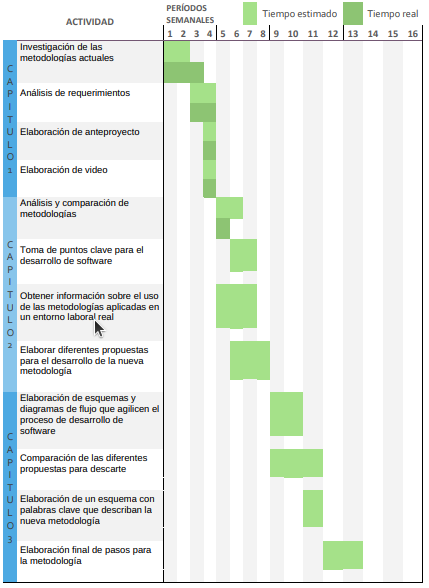
\includegraphics[width=.8\textwidth]{cronograma}
	%\includegraphics[scale=4]{image}
	\caption{Cronograma de Actividades}
	\label{fig:etiquetafigura}
\end{figure}

\end{document}